\section{Upgrades} 
In this chapter we will explain how upgrades are implemented in the game. We 
will go through some of the code and show the design patterns we used.

\subsection{Implementation} 
\label{Upgrades} 
Players can purchase upgrades for different entities. E.g. the player can 
upgrade the carrying capacity, which doubles the carrying capacity of workers. 
Upgrades can be found in the research building. The upgrade system has its own 
panel, however it is identical to the entity panel (\cref{sec:EntityPanel}), 
so we won't go into further detail on how the panel works in this chapter. 

The upgrade system makes use of an upgrade manager. This class is a singleton.
It keeps track of which upgrades have been bought and it has a collection of
all possible upgrades. At the moment there are four upgrades.

\begin{enumerate} 
    \item Carrying Capacity - doubles carrying capacity 
    \item Gather Speed - doubles gather speed 
    \item Health - increases HP of all units with 15\% 
    \item Attack Damage - increases attack damage of all units with 15\% 
\end{enumerate}

\begin{figure}[H] 
    \centering 
    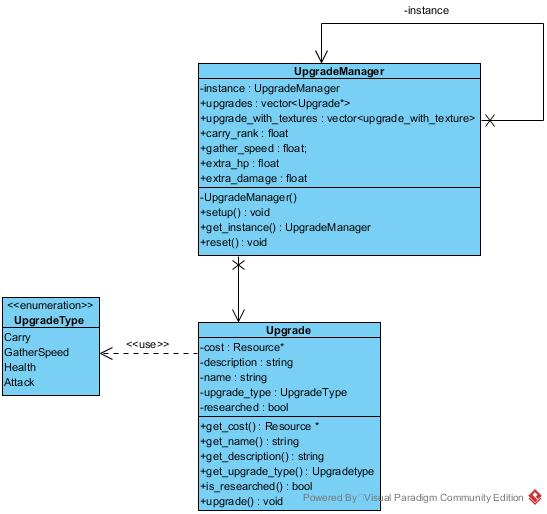
\includegraphics[scale=0.75]{res/upgrades.jpg}
    \caption{Upgrade class diagram.}\label{fig:upgrade-figure} 
\end{figure}

When a player purchases an upgrade, the upgrade method of Upgrade will
be called. In this method we check if the player has enough resources and after
that we check which upgrade has been selected and activate the corresponding
upgrade. 

\begin{lstlisting} 
case UpgradeType::Health:
    UpgradeManager::get_instance()->extra_hp = 1.15; 
    for (int i = 0; i < PlayerManager::get_instance()->get_player(player_id)->units.size(); i++) {
        PlayerManager::get_instance()->get_player(player_id)->units.at(i)->upgrade_health();
    } 
    break; 
\end{lstlisting}

As you can see in the code above, the variable extra\_hp is set to 1.15. This
variable is used in the constructor of all concrete implementations of
MovingEntities. E.g. a knight normally has 125 health, we multiply this with
extra\_hp. So without an upgrade the health stays the same, but once a player
has bought an upgrade health and max\_health are multiplied by 1.15. We also
have to upgrade the health for all existing MovingEntities of the player, which
can also be seen in the code fragment.

This is a code fragment from the constructor of the knight entity.
\begin{lstlisting} 
_max_health = 125 * UpgradeManager::get_instance()->extra_hp; 
_health = 125 * UpgradeManager::get_instance()->extra_hp; 
\end{lstlisting}


This is what the upgrade panel looks like.

\begin{figure}[H] 
    \centering 
    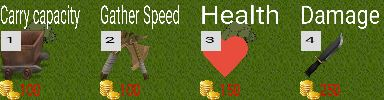
\includegraphics{res/up.jpg} 
    \caption{No upgrades bought yet.} 
\end{figure}

\begin{figure}[H] 
    \centering 
    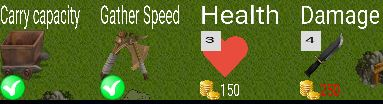
\includegraphics{res/up2.jpg} 
    \caption{Two upgrades bought.} 
\end{figure}
